\section{Evaluation}
\label{sec:eval}
%
This section describes our experience running \helix in production at \linkedin and
then presents experiments demonstrating \helix's functionality and production.

\subsection{\helix at \linkedin}
\label{sec:production}
%
From the beginning we built \helix for general purpose use, targeting \ES, \seas
and \databus.  As mentioned earlier, we chose these systems
to ensure \helix became a truly general cluster manager and not, say, a
cluster manager for distributed databases. 
The systems were themselves under development and in need of cluster management
functionality, and so were likewise attracted to \helix.
At the time of this writing, all three of \ES, \seas and \databus run in
production supported by \helix.

With every \helix-DDS integration we found and repaired gaps in the \helix
design, while maintaining its generality.  For example, \seas needed more
control than auto replica placement offers, and so we added semi-auto and
custom modes.
We also added a \emph{zone} concept to support grouping a set of
nodes together.  This is useful, for example, in rack-aware replica placement
strategies.  

The first \helix version did not include constraints and goals on transitions, but instead
satisfied this requirement by overloading state constraints and goals.  This complicated
the algorithms for computing and throttling transitions.  We added support for
throttling transitions at different cluster granularities to remove this
complexity.

\eat{%%%%%%%
\helix's generic model of a DDS cluster has indeed given us the ability to
greatly accelerate the cluster management aspects of DDS development.  A great
example came from experimenting with different replication designs for \ES.  One
preliminary design we tried was to use native
\mysql-based
replication to synchronize slave replicas with masters, rather than
\databus-based replication.  \aes{briefly explain why mysql-based is not as
good. Kishore: Kapil can you fill this up ?}  

The \ES changes needed to
integrate with \mysql replication took a
considerable amount of time, but the cluster management changes were nearly
trivial.  One change for this version of \ES is that it required each node to contain only masters or only
saves.  We did not have to change its state model but rather only changed its
placement optimization goals to achieve this.  This stresses the value of
\helix's pluggable design. 
A second change was to have each slave-only node in the cluster know its
partitions' masters, in order to initiate replication.  We added no \ES code to
support this communication, but instead simply added the spectator role to each
\ES node.   This shows the value we gain from the \helix roles and being able to
flexibly combine them.
}%%%%%%%%%%

\textbf{DDS debugging and correctness checking}
%
One of the most interesting benefits of \helix falls out of its ability to
manage a cluster without specific knowledge of the DDS's
functionality by allowing the DDS
to express them in the form of AFSM and constraints and optimization goals. We
have built a debugging tool capable to analyzing a DDS's correctness.
Testing distributed systems is extremely difficult and laborious, and it cannot
be done with simple unit tests.   Generic
debugging tools that function in the distributed setting are especially valuable.  

Our tool uses the ''instrument,
simulate, analyze'' methodology. This consists of
\squishlist
\item \textbf{Instrument} Insert probes that provide information about the state of the system
over time.  We use Zookeeper logs as ''probes.''
\item \textbf{Simulate} We use robots to create cluster error, killing
components and injecting faults, both on the DDS and \helix sides.
\item \textbf{Analyze} We parse the logs into a relational format, load them into a database as
a set of tables and then write invariants on the DDS's constraints.  Violation
of the constraints signals a possible bug.
\squishend

Every DDS that uses \helix automatically benefits from this tool and it has been crucial
in improving performance and debugging production issues.  
One of the most difficult parts of debugging a DDS is understanding the sequence
of events that leads to failure.  \helix logging plus the debugging tool make it
easy to collect system information and reconstruct the exact sequence of
events that lead to the failure.
As a concrete example, the experiment on
planned downtime we describe in Section~\ref{sec:downtime} uses this tool to
measure total downtime and partition availability during software upgrades.
This lets us experiment with different upgrade policies and ensure they are
performant and valid.

\eat{%%%%%%%
One of the most interesting and useful benefits of \helix is its ability to
analyze a DDS's correctness without having any specific knowledge of the DDS's
functionality.  \aes{Ramesh to describe how we have built tools to co-analyze a
log and a state model to check for correctness, how often a DDS is in
violation.}  \aes{Introduce experiment in this area.}  \aes{Show a graph of tool
in practice.}  \aes{Describe result...since this is now in the production
experience section, tone should be how this helps us write/test/deploy DDSs.}
\aes{Make sure to point out that violations do not necessarily mean bugs...just
a little is unavoidable, more than a little could be a design issue, lots could
be a bug.  This tools helps the designer figure gives them insight into DDS so
they can figure it out.}
}%%%%%%%%%%%%

\subsection{Experiments}
\label{sec:experiments}
%
Our experiments draw from a combination of production and experimental
environments, using the DDS \ES.  The clusters are built from
production-class commodity \\ servers.  The details of the production
clusters are confidential, but we present details on our experimental cluster 
throughout our experiment discussion. 

\eat{%%%%%%%
Throughout the experiments we vary different parameters of \helix and
\ES.
We default to the following settings and list changes with each experiment. 
\aes{Kishore to put in a single default value for each param}
\begin{table}
\begin{tabular}{| l | l | }
\hline  Transition Execution Time & 100ms  \\ 
\hline  Replicas & 3 \\
\hline
\end{tabular}
\end{table}
}%%%%%%

\subsubsection{Bootstrap}
\label{sec:bootstrap}
%

\begin{figure*}[t]
  \begin{minipage}[t]{0.48\textwidth}
    {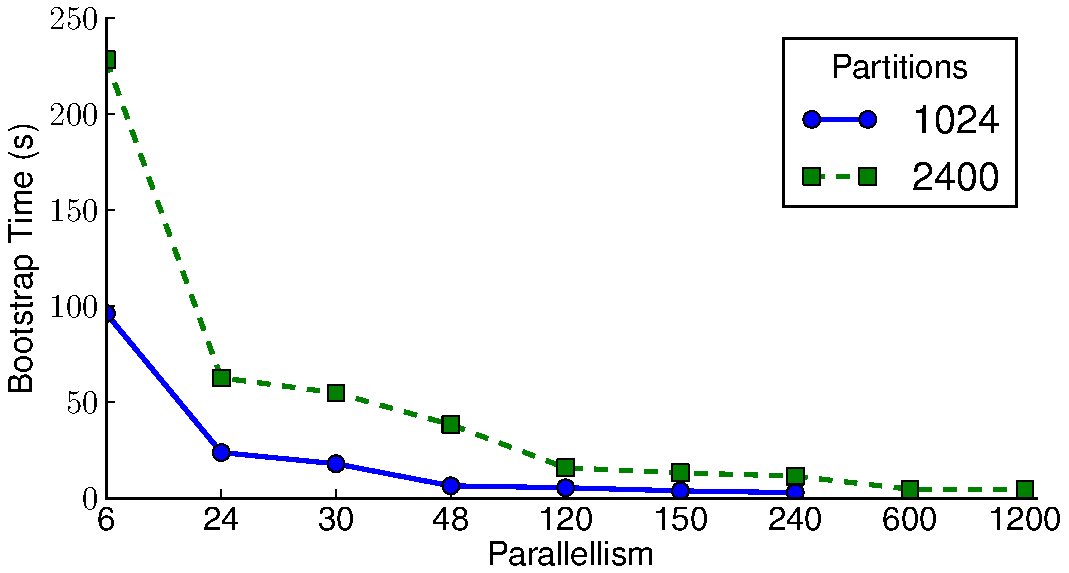
\includegraphics[width=0.90\textwidth]{bootstrap.pdf}}
    \vspace*{-2ex}
    \caption{\label{fig:bootstrap_time} \ES transition parallelism vs. bootstrap time.}
  \end{minipage}
  \hfill
  \begin{minipage}[t]{0.48\textwidth}
    {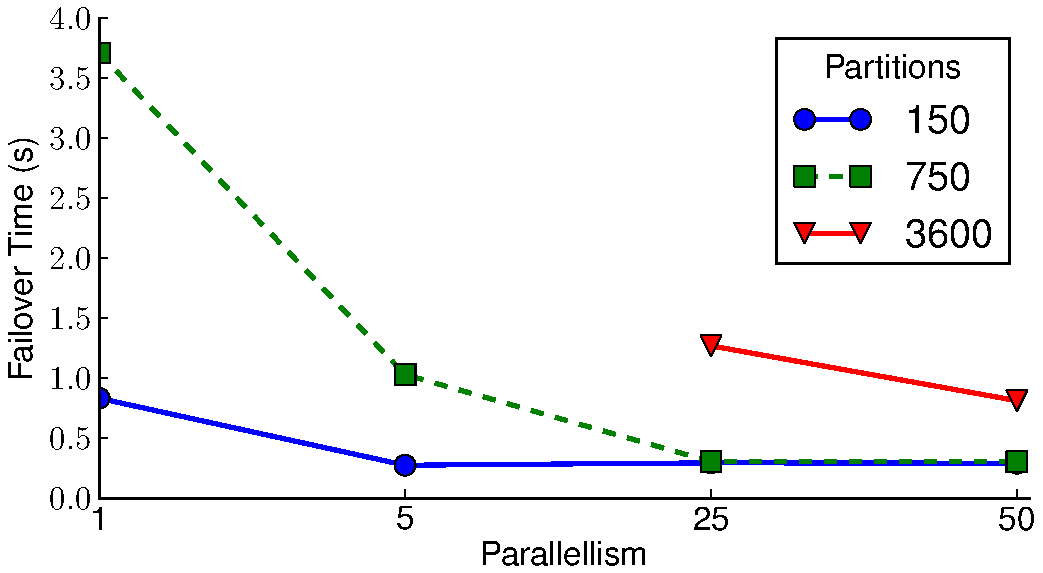
\includegraphics[width=0.90\textwidth]{failure.pdf}}
    \vspace*{-2ex}
    \caption{\label{fig:failure_detection} \ES transition parallelism vs. failover time.}
    \end{minipage}
    \vspace*{-2ex}
\end{figure*}


\eat{%%%%%%%
\begin{figure}[t]
    {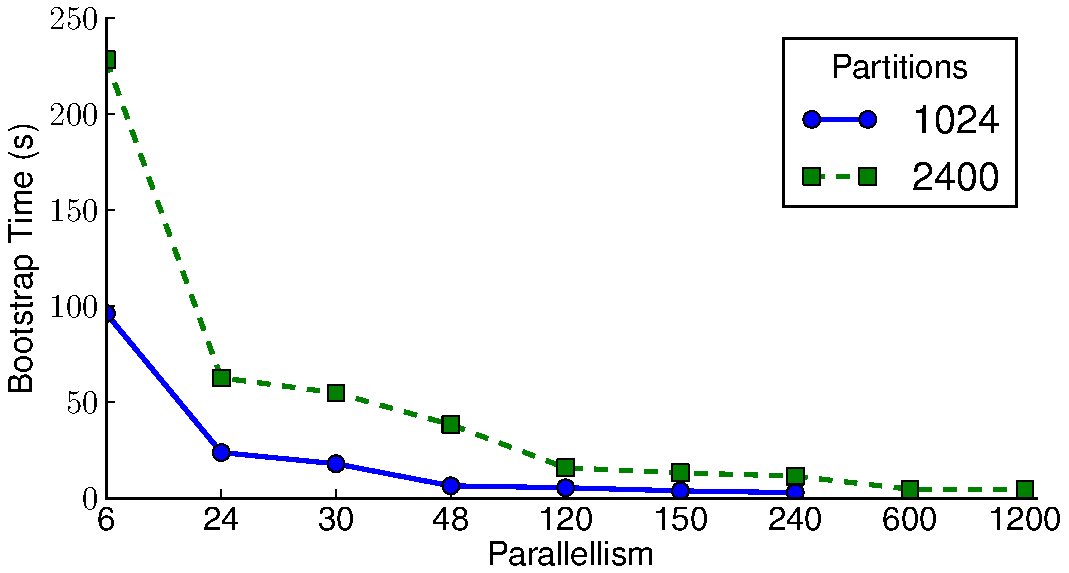
\includegraphics[width=\columnwidth]{bootstrap.pdf}}
    \vspace*{-2ex}
    \caption{\label{fig:bootstrap_time} \ES bootstrap time v/s parallelism.}
\end{figure}
}%%%%%%%%


Our first experiment examines \helix's performance when bootstrapping an \ES cluster,
(\ie adding the initial nodes and databases).  We note that while for some DDSs
bootstrapping is a rare operation, for others, like \databus consumers, it
happens frequently, and fast bootstrap times are crucial.

We vary the number of allowed parallel transitions, add nodes and an \ES
database, and then measure the time taken for the cluster to reach a stable
state.  We repeat the experiment for 1024 partition and 2400 partition
databases. 
Figure~\ref{fig:bootstrap_time} plots the result and shows that bootstrap time
decreases with greater transition parallelism, though the benefits diminish once
parallelism is in the tens of transitions.

The total bootstrap time is directly proportional to the number of transitions
required and inversely proportional to the allowed parallelism.  The number of
required transitions is a function of the number of partitions, number of
replicas per partition and the transitions drawn from \ES's state machine.
For example, an Espresso database with $p$ partitions and $r$ replicas requires
$pr$ offline$\rightarrow$slave transitions and $p$ slave$\rightarrow$master
transitions.  \ES sets allowed parallelism based on the number of cluster nodes
and the number of concurrent transitions a node can handle.
The final factor in deriving bootstrap time is the time required to execute each
individual transition.  These times are DDS dependent. 
For example, when an \ES partition enters the slave state \ES creates a \mysql
database and all required tables for it; this takes tens of milliseconds.
On bootstrap, this transition takes approximately 100 ms.  

Although it is obvious that improving the parallelism in transitions will
improve the time to bootstrap, overhead added by \helix is proportional to the
number of transitions that can be executed in parallel. Through experiments we
found the majority of this time is spent updating cluster metadata in
Zookeeper. \helix employs many techniques to minimize this time,like asynchronous 
writes to Zookeeper, restricting writes to a Zookeeper node to a single process to avoid
conflicts, and a group commit protocol to allow multiple updates to one
Zookeeper.

The graphs depict that even as we increase the number of partitions, by
increasing parallelism, \helix is able to close the gap in
bootstrap time. The gap is larger at low parallelism because the benefit from techniques like
group commit kick in when parallelism is high. We also see that increasing
parallelism eventually does not further lower bootstrap time.

\subsubsection{Failure Detection}
\label{sec:failuredetection}
%
One of \helix's key requirements is failure detection, and its performance in
this area must match what a DDS might achieve for itself with a custom solution.
In \ES, losing a node means all partitions mastered on that node become
unavailable for write, until \helix detects the failure and promotes slave
replicas on other nodes to become masters.
\eat{%%%%%%%
\begin{figure}[t]
    {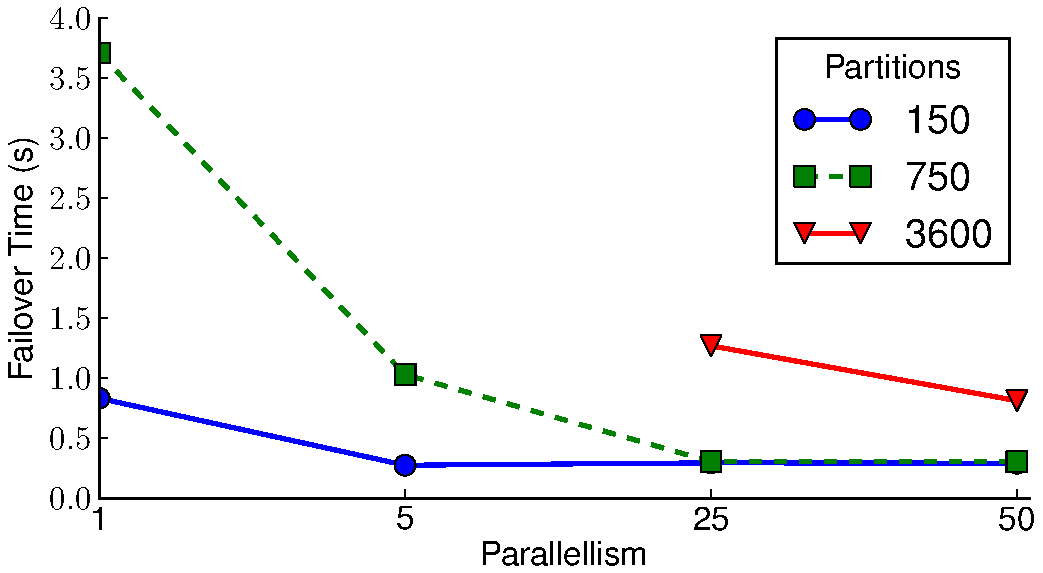
\includegraphics[width=\columnwidth]{failure.pdf}}
    \vspace*{-2ex}
    \caption{\label{fig:failure_detection} Failover time v/s parallelism}
\end{figure}
}%%%%%%%%%%
We run an experiment with an \ES cluster of size 6, randomly kill a single
node, and measure write unavailability.  We vary the the number
of \ES partitions and the maximum cluster-wide allowed parallel transitions.
Figure~\ref{fig:failure_detection} plots the result and shows most importantly
that we achieve low unavailability in the 100s of ms, and that this time decreases as we allow
for more parallel transitions.  It is interesting to note that earlier versions
of \helix had recovery times of multiple seconds.  The reason is that when so
many partitions transitioned from slave to master at once, \helix actually
bottlenecked trying to record these transitions in Zookeeper.  We ultimately
solved that bottleneck using techniques like group commit and asynchronous
reads/writes;  the key point is that we solved this problem for every DDS using \helix and masked
internal Zookeeper details from them.    

\subsubsection{Elastic Cluster Expansion}
\label{sec:elastic}
%
\begin{figure}[t]
    {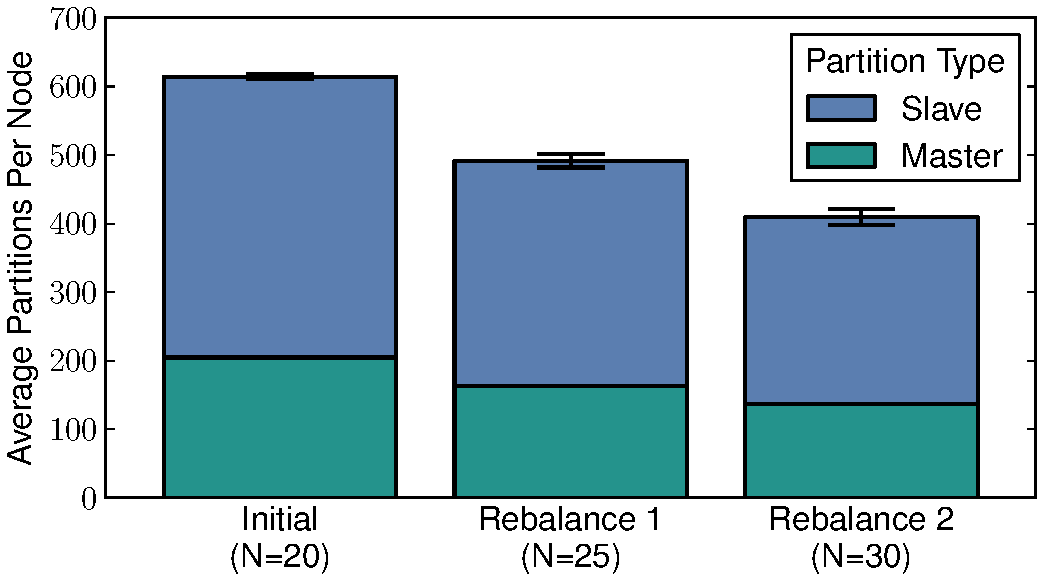
\includegraphics[width=\columnwidth]{rebalance.pdf}}
    \vspace*{-2ex}
    \caption{\label{fig:cluster_expansion} Elastic Cluster Expansion }
\end{figure}

Another of \helix's key requirements is its ability to incorporate new nodes as
clusters expand.  Recall Algorithm~\ref{alg:execution}
handles moving partitions from existing to new nodes by computing target
states. 
We want to ensure rebalancing moves as few replicas as possible; in
particular, in \ES, we want to ensure that the number of replicas moved is
minimized, since these involve transitions that copy data from node to another
which is expensive.
We run an experiment that starts with a cluster with 20 nodes,
4096 partitions and 3 replicas per partition. We then add 5 new nodes, Helix
recalculates the placement and we find that 19.6\% of partitions are moved.  The
optimal percentage moved for full balance is clearly 20\%; with this
experiment's server and partition counts, achieving 20\% movement requires
moving partition fractions and so we instead achieve near balance.

Finally, we add an additional 5 nodes. After \helix recalculates the
placement we see that 16\% of partitions are moved, close to the optimal
solution. 
Figure~\ref{fig:cluster_expansion} shows we are minimal in
the number of partitions moved to ensure even load distribution.
While RUSH is very good at accomplishing this type of balancing, RUSH does not inherently support the 
concept of different replica states and is by default
designed for handling numbers of partitions that are orders of magnitude greater
than the number of nodes.  As discussed in Section~\ref{sec:design} we modified it to handle different states and
possibly much smaller numbers of partitions and still achieve close to minimal
movement.

\subsubsection{Planned upgrade}
\label{sec:downtime}
%
One function that \helix manages for DDSs is planned downtime, which helps for a
variety of administrative tasks, such as server upgrades.  In \ES bringing down
a node involves moving every partition on it to the offline state and
transitioning partitions on other servers to compensate. In fact, there
is a direct tradeoff between total time to complete planned downtime (\eg to
upgrade all nodes) versus accumulated unavailability over that time. 

Since Helix provides fault tolerance, a DDS system can upgrade its software by upgrading one node at a time. 
The goal of this exercise is to choose a reasonable tradeoff between minimizing
total upgrade time and minimizing unavailability during the upgrade. 
One simple approach is to upgrade one node at a time. 
Though this approach is common, it may in reality reduce the availability of the
system. 

In this experiment we showcase the impact of concurrent partition migration on a
single node. We fix the total number of migrations at 1000 and control the
batch size of partitions that may be concurrently migrated. 

What we see in this experiment is when 100 percent partitions are migrated
 concurrently, the variation in downtime per partition is very high compared to
 the variation when 25 percent of partitions are migrated. The unavailability is
 measured as the sum total of unavailability for each partition. The ideal
 percentage of partitions to chose for upgrade is directly proportional to the
 maximum transitions that can concurrently occur on a single node. The purpose
 of this experiment is to demonstrate that \helix provides a DDS the ability experiment
 with various percentages and choose the one where unavailability is minimized.

\begin{figure}[t]
    {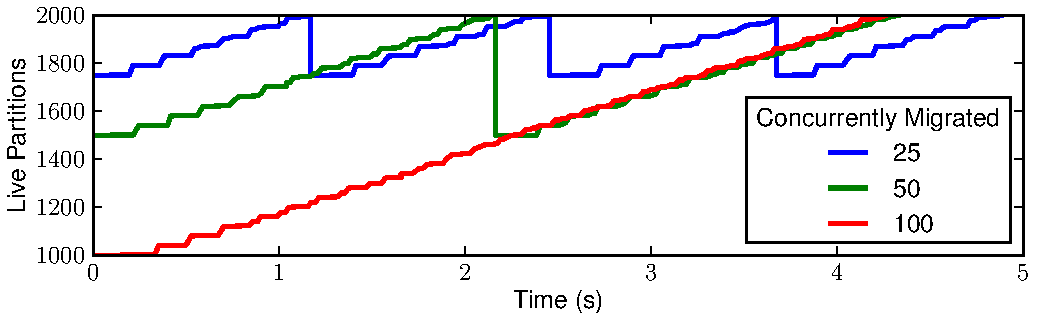
\includegraphics[width=\columnwidth]{migration-timeseries.pdf}}
    \vspace*{-2ex}
    \caption{\label{fig:migration_timeseries} Percentage of partitions that are
available over the course of a planned software upgrade.}
\end{figure}

\begin{figure}[t]
    {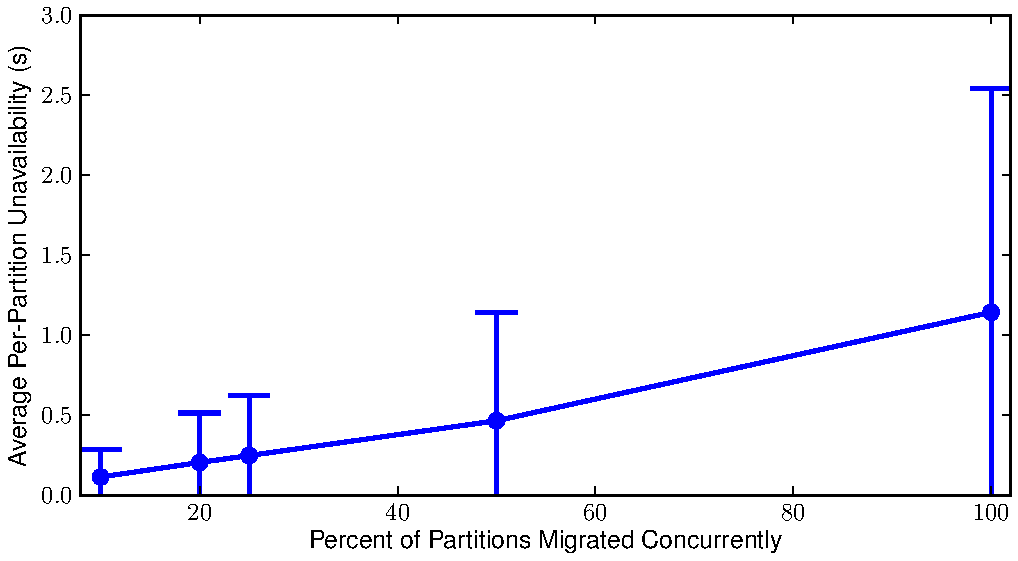
\includegraphics[width=\columnwidth]{average-migration.pdf}}
    \vspace*{-2ex}
    \caption{\label{fig:average_timeseries} Average unavailability per partition
during planned software upgrade.}
\end{figure} 

Figure~\ref{fig:migration_timeseries} shows that by choosing a lower concurrency
level, each migration is faster but the overall time taken to upgrade a node is larger.

Figure~\ref{fig:average_timeseries} shows a different perspective by plotting
the average per partition unavailability. It also shows that the variance grows
quite high as parallelism increases. While lower upgrade times are appealing,
higher error counts during upgrades are not.

The ability to balance downtime and unavailability is important for DDSs so the
upgrade process becomes smooth and predictable.  Beyond what is illustrated in
the scope of this experiment we also see cases where throttling transitions is
important to avoid load spikes that also affect availability.  For example,
bringing up too many \ES partitions online at the same time, when they have cold
caches, will cause failures.  By controlling transitions at the partition
granularity, \helix helps DDSs avoid availability and performance problems, and
manage planned downtime duration.

\begin{figure*}[t]
  \begin{minipage}[t]{0.48\textwidth}
    {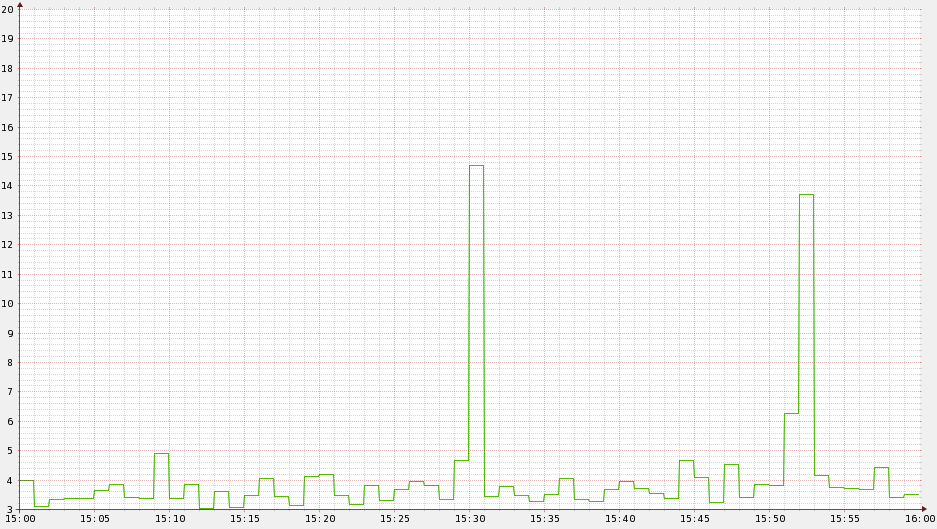
\includegraphics[width=0.99\textwidth]{expr/alert_graphs/latency99th_app74_alert_value.png}}
    \vspace*{-2ex}
    \caption{\label{fig:latency_alert} Alert reporting 99th percentile latency
on a single \ES node.}
  \end{minipage}
  \hfill
  \begin{minipage}[t]{0.48\textwidth}
    {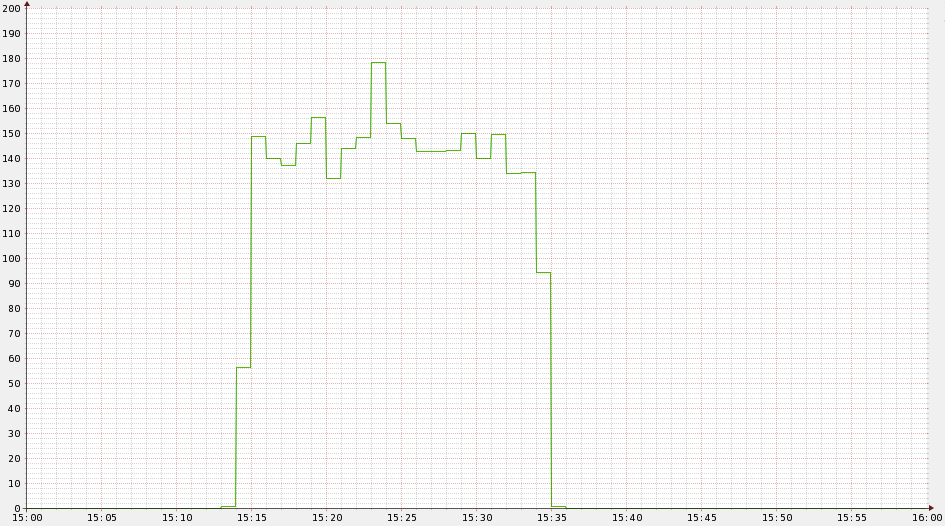
\includegraphics[width=0.99\textwidth]{expr/alert_graphs/errorcount_sumeach_alert_val.png}}
    \vspace*{-2ex}
    \caption{\label{fig:error_alert} Alert reporting the cluster-wide \ES error count.}
    \end{minipage}
    \vspace*{-2ex}
\end{figure*}

\subsubsection{Alerts}
%
Recall from Section~\ref{sec:design} that \helix provides DDSs a framework for
defining monitored statistics and alerts.  Here we give some examples of alerts
\ES runs in production.

\ES monitors request latency to ensure it is meeting its SLAs or take
corrective action otherwise.  Specifically it registers the alert \\
\texttt{decay(1)(node*.latency99th) > 100ms}  \\
Since the alert is wildcarded on node name, we separately monitor 99th
percentile latency on each node in the \ES cluster.  The decaying sum setting of 1
means we monitor the latest reported value from each node, and ignore older
values.  Figure~\ref{fig:latency_alert} shows a production graph displaying the current monitored value for a
particular \ES node.  The x and y axes are wall time and request latency,
respectively.  A similar graph (not shown here) indicates whether the
alert is actually firing and, when fired, emails notification to \ES operators.

A second alert monitors the cluster-wide wide request error count: \\
\texttt{decay(1)(node*.errorcount)|SUMEACH > 50ms}  \\
The alert is again wildcarded on node name, but now computes the sum of errors
over all nodes.  Figure~\ref{fig:error_alert} shows the production graph and,
again, there is an unshown corresponding graph displaying the alert status.

%Template for displaying graphs
\eat{%%%%%%%%%%
\begin{figure*}[t]
  \begin{minipage}[t]{0.48\textwidth}
    {\includegraphics[width=0.85\textwidth]{experiments/load/load1K.eps}}
    \vspace*{-2ex}
    \caption{\label{fig:load1K} Load times for 120 million 1K records.}
  \end{minipage}
  \hfill
  \begin{minipage}[t]{0.48\textwidth}
    {\includegraphics[width=0.85\textwidth]{experiments/load/vary_rec_size.eps}}
    \vspace*{-2ex}
    \caption{\label{fig:vary-rec-size} Load times for 120GB, varied record
size.}
    \end{minipage}
    \vspace*{-2ex}
\end{figure*}
}%%%%%%%%%
